\section{Charged-Current Inclusive Electron Neutrino Selection }
\label{sec:nueselection:inclusive}

\newcommand{\pct}[1]{\SI{#1}{\%}}
\newcommand{\syst}{systematic uncertainty\xspace}
\newcommand{\systs}{systematic uncertainties\xspace}
\newcommand{\unbpot}{\SI{5.5e19}{POT}\xspace}
\newcommand{\fullpot}{\SI{6.9e20}{POT}\xspace}

The inclusive charged-current electron neutrino selection aims to minimise selection bias towards either the neutrino energy or the topology of the event. The selection efficiency is \pct{18.1+-0.1} (stat.), leading to approximately 200 electron neutrino's in the Run 1-3 data-set of \fullpot. The expected distribution of selected event after selection is given in \cref{fig:nuecc:expected}. The estimated \nuecc purity is \pct{54.0+-1.0}.

\begin{figure}[H]
    \centering
    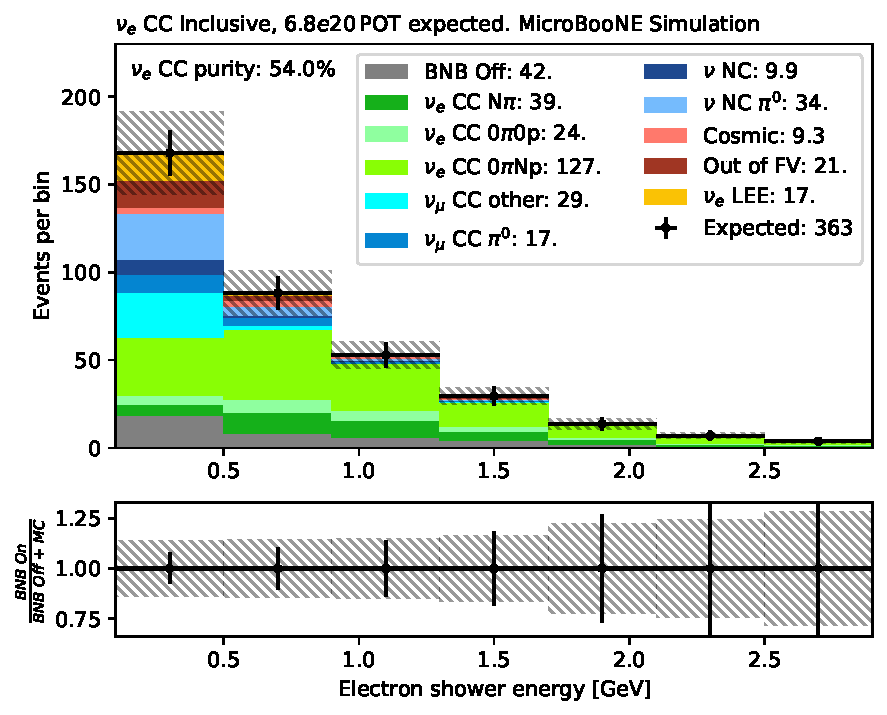
\includegraphics[width = 0.5\textwidth]{NueCCsel/Images/truth/intro_plot_scaled.pdf}
    \caption{Expected event spectrum for the \nuecc selection, scaled to the \fullpot Run 1-3 data-set. The expected data is shown to indicate the relative size between the statistical fluctuations and \systs. As is valid for all plots in this chapter, unless stated otherwise, the hatched error bar includes the systematic uncertainties arising from flux, cross-section modelling (GENIE), Geant re-interactions and detector variations.}
    \label{fig:nuecc:expected}
\end{figure}

While this selection is not designed to provide sensitivity to the MB-$\nu_e$ LEE model (\cref{sec:introduction:LEE}), it is able to achieve higher efficiency and purity compared to the exclusive channels, particularly at high energy, and as such plays an important role in measuring and validating the intrinsic $\nu_e$ model prediction. Additionally, because the selection does not differentiate based on topology of electron kinematics, it is suited to perform such measurements after selection with higher statistics. The selection strategy is introduced in \cref{fig:nue_flow}. 

The effect of \systs on the efficiency and distributions will be discussed in \cref{sc:nuecc:syst}. Unless explicitly stated otherwise; uncertainties from simulation statistics, flux, cross-section modelling (GENIE), Geant re-interactions and detector variations are included in every plot in this chapter as hatched error bars.

The results of the high-energy far-sideband are described in \cref{sc:nuecc:sideband}. In this chapter, comparisons with the usual \unbpot Unbiased open data-set will be given. 

\begin{figure}[htb]
    \centering
    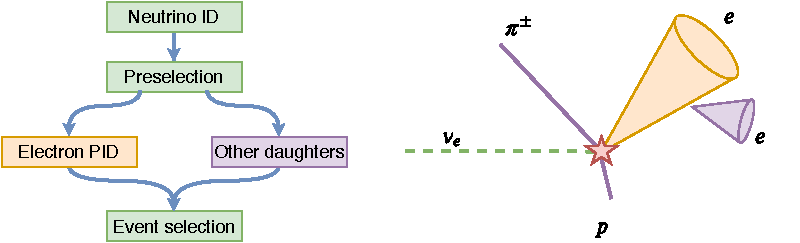
\includegraphics[width = 0.8\textwidth]{NueCCsel/Images/nueccflow}
    \caption[Flowchart indicating the different steps in the \nuecc selection]{(Left) Flowchart indicating the different steps in the \nuecc selection. (Right) A schematic representation of a \nuecc event with multiple reconstructed showers and tracks. At the preselection stage (\cref{sc:nuecc:presel}), an electron candidate shower is identified (orange) and electron particle identification (\cref{sc:nuecc:e_pid}) is performed on this shower. The other reconstructed objects (purple) are classified (\cref{sc:nuecc:d_pid}) to improve background rejection before merging the outputs and perform the final event selection (\cref{sc:nuecc:sel}).}
    \label{fig:nue_flow}
\end{figure}

\subsection{Preselection}
\label{sc:nuecc:presel}


The preselection builds on top of the NeutrinoID (\cref{sec:sliceID}). The cuts listed in \cref{tab:nuecc:presel} are applied.

\begin{comment}
\begin{figure}[htb]
\begin{center}
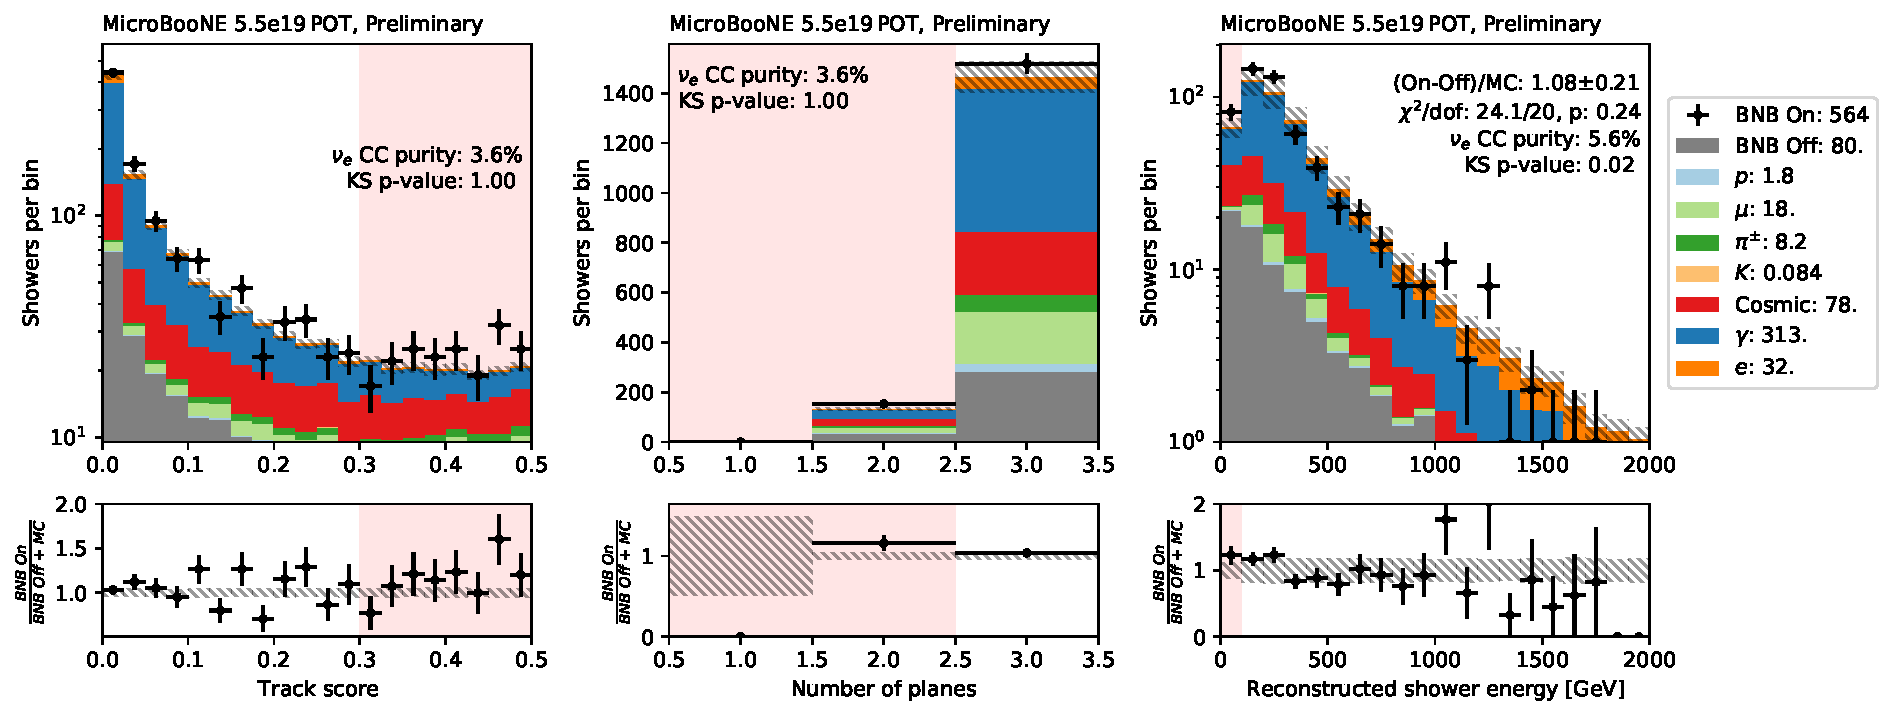
\includegraphics[height=0.27\textheight]{NueCCsel/Images/datamc/presel_2.pdf}
\end{center}
\caption[Electron shower candidate identification in the \nuecc selection]{(Left) The track score as described in \cref{sec:NuEvtReco} The histogram is filled for all objects passing the reconstruction-based quality requirements (see text for details). Objects with a low track score are more shower-like. (Right) The reconstructed shower energy obtained from the deposited charge on the collection plane. The histogram is filled with all showers passing the topological score cut and previous requirements. The bin size on the $x$-axis is \SI{50}{\MeV}. Events in the shaded red region are rejected. Both cuts aim to select electron showers. Note the logarithmic scale on the vertical axis in both panels.}
\label{fig:trk_she}
\end{figure}
\end{comment}

\begin{table}[htb]
\centering
\setlength{\tabcolsep}{10pt}
\renewcommand{\arraystretch}{1.25}
\begin{tabular}{|c|c|}
\hline
Cut goal                          & Cut definition                                                              \\ \hline \hline
\multirow{5}{*}{Cosmic rejection} & Selected by the NeutrinoID (\cref{sec:sliceID})                                 \\
                                  & Reconstructed neutrino vertex is in fiducial volume (\cref{fig:nuecc:fidvol})\\
                                  & Topological score $>$ 0.15 (\cref{fig:nuecc:presel_1}, left)                 \\
                                  & CosmicIPAll3D $>$ 30 \si{\cm}   (\cref{fig:nuecc:presel_1}, middle)          \\
                                  & $\mid$CosmicDirAll3D$\mid$ $<$ 0.98     (\cref{fig:nuecc:presel_1}, right)   \\ \hline
\multirow{5}{*}{Signal topology}  & Object with most hits is shower-like                                         \\                                    & Electron shower candidate: \\
                                  &      \tabitem Track score below 0.3 (\cref{fig:nuecc:presel_2}, left) \\
                                  &     \tabitem Reconstructed hits on three planes (\cref{fig:nuecc:presel_2}, middle) \\
                                &        \tabitem Minimum \SI{100}{\MeV} shower energy (\cref{fig:nuecc:presel_2}, right) \\ \hline
\end{tabular}
\caption{\label{tab:nuecc:presel} Preselection requirements for the \nuecc inclusive selection.}
\end{table}


At this stage, the efficiency of the selection is \pct{36.3+-0.2} for $\nu_e$ CC events inside the fiducial volume. The purity of \nuecc events in the preselection is \pct{6.28+-0.04}. The angular distributions of the identified electron candidate is shown in \cref{fig:nuecc:theta_phi}.

\begin{figure}[htb]
    \centering
    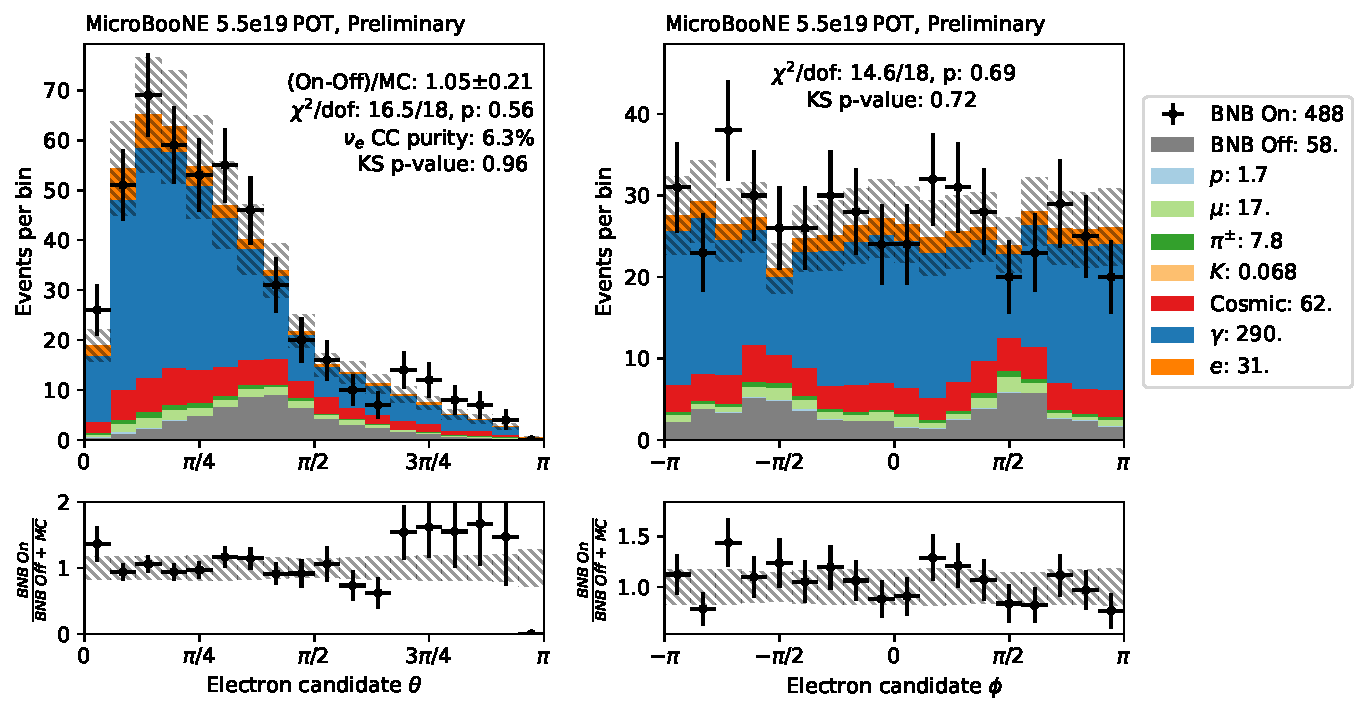
\includegraphics[height=0.27\textheight]{NueCCsel/Images/datamc/e_cand_theta_phi.pdf}
    \caption[Electron shower candidate $\theta$ and $\phi$ angles after the preselection]{Electron shower candidate $\theta$ (left) and $\phi$ (right) angular distributions after the preselection. The histogram is categorised using the reco-truth matched particle type corresponding to the electron candidate shower.}
    \label{fig:nuecc:theta_phi}
\end{figure}

\subsection{Electron Identification}
\label{sc:nuecc:e_pid}

After the preselection, the object tagged as the electron candidate is still not a neutrino-induced electron in most events. The ratio of photons to electrons is approximately 9 to 1 (see for example \cref{fig:nuecc:theta_phi}), and $e$/$\gamma$ separation is therefore the main objective of electron identification. The identification is done using a boosted decision tree (XGBoost), trained on the variables listed in \cref{tab:nuecc:e_bdt}. The two variables with the largest separation power are shown in \cref{fig:e_cand_1}.

\begin{figure}[htb] 
    \centering
    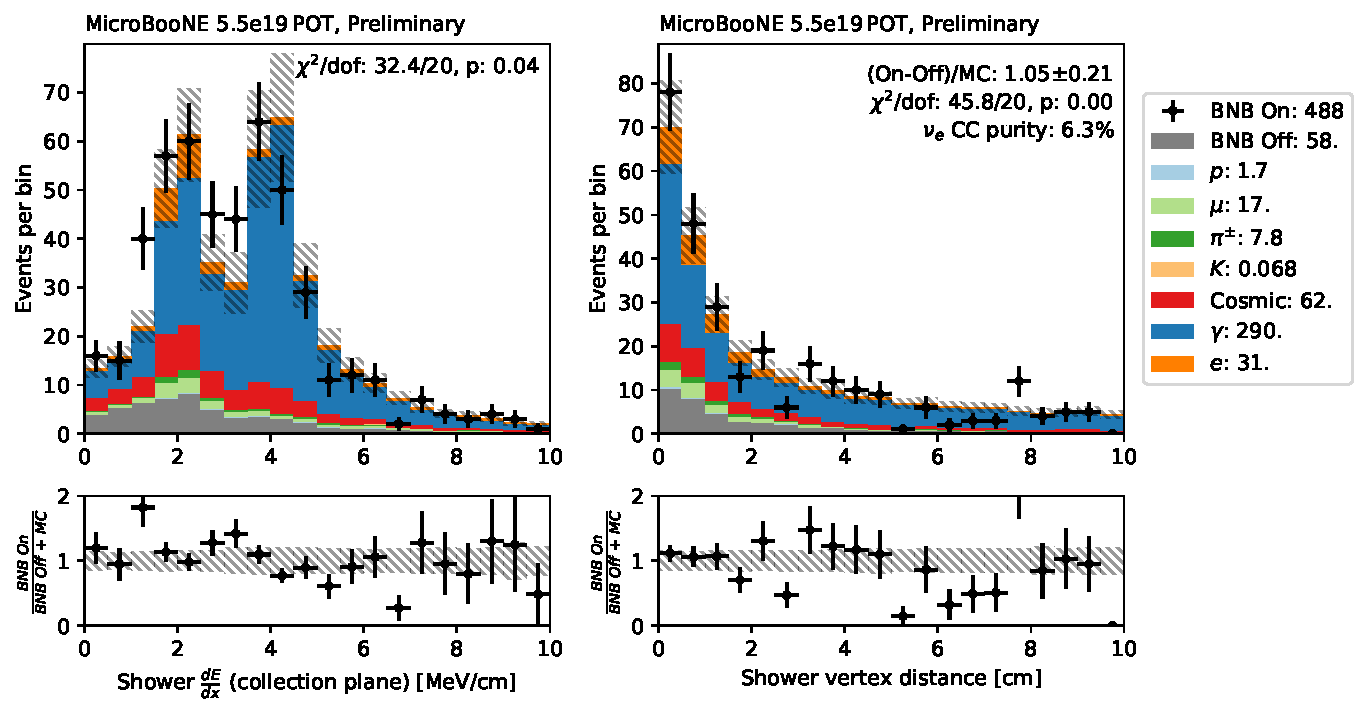
\includegraphics[height=0.27\textheight]{NueCCsel/Images/datamc/e_cand_1.pdf}
    \caption{\label{fig:e_cand_1} The two electron candidate shower variables with the cleanest electron-gamma separation: The \dedx on the collection plane in the first \SI{4}{\cm} of the shower (left) and the vertex distance between the shower start and the reconstructed neutrino interaction point (right).}
\end{figure}

\par
The binary classification tree tries to distinguish backtracked electron showers from background showers, dominated by photons. The training and testing if fully performed on a cocktail of simulated overlay events, and no data events are used in the training. This mixture consists mostly of BNB-like neutrino events, enriched with electron neutrino interactions and weighted to compensate the energy dependence of the beam flux. 
\par
The outcome of the training process -- the BDT response -- and validation is given in \cref{fig:nuecc:train_e}. The data/MC comparison of both the remaining input variables and the response of the BDT are shown in \cref{fig:nuecc:e_cand_all}. The correlation between the variables used to obtain the electron identification score, the score itself, the reconstructed lepton kinematics and the simulated-based lepton kinematics are shown for \nuecc electrons, passing the preselection in \cref{fig:nuecc:corr_electrons}.

\begin{figure}[htb]
\centering
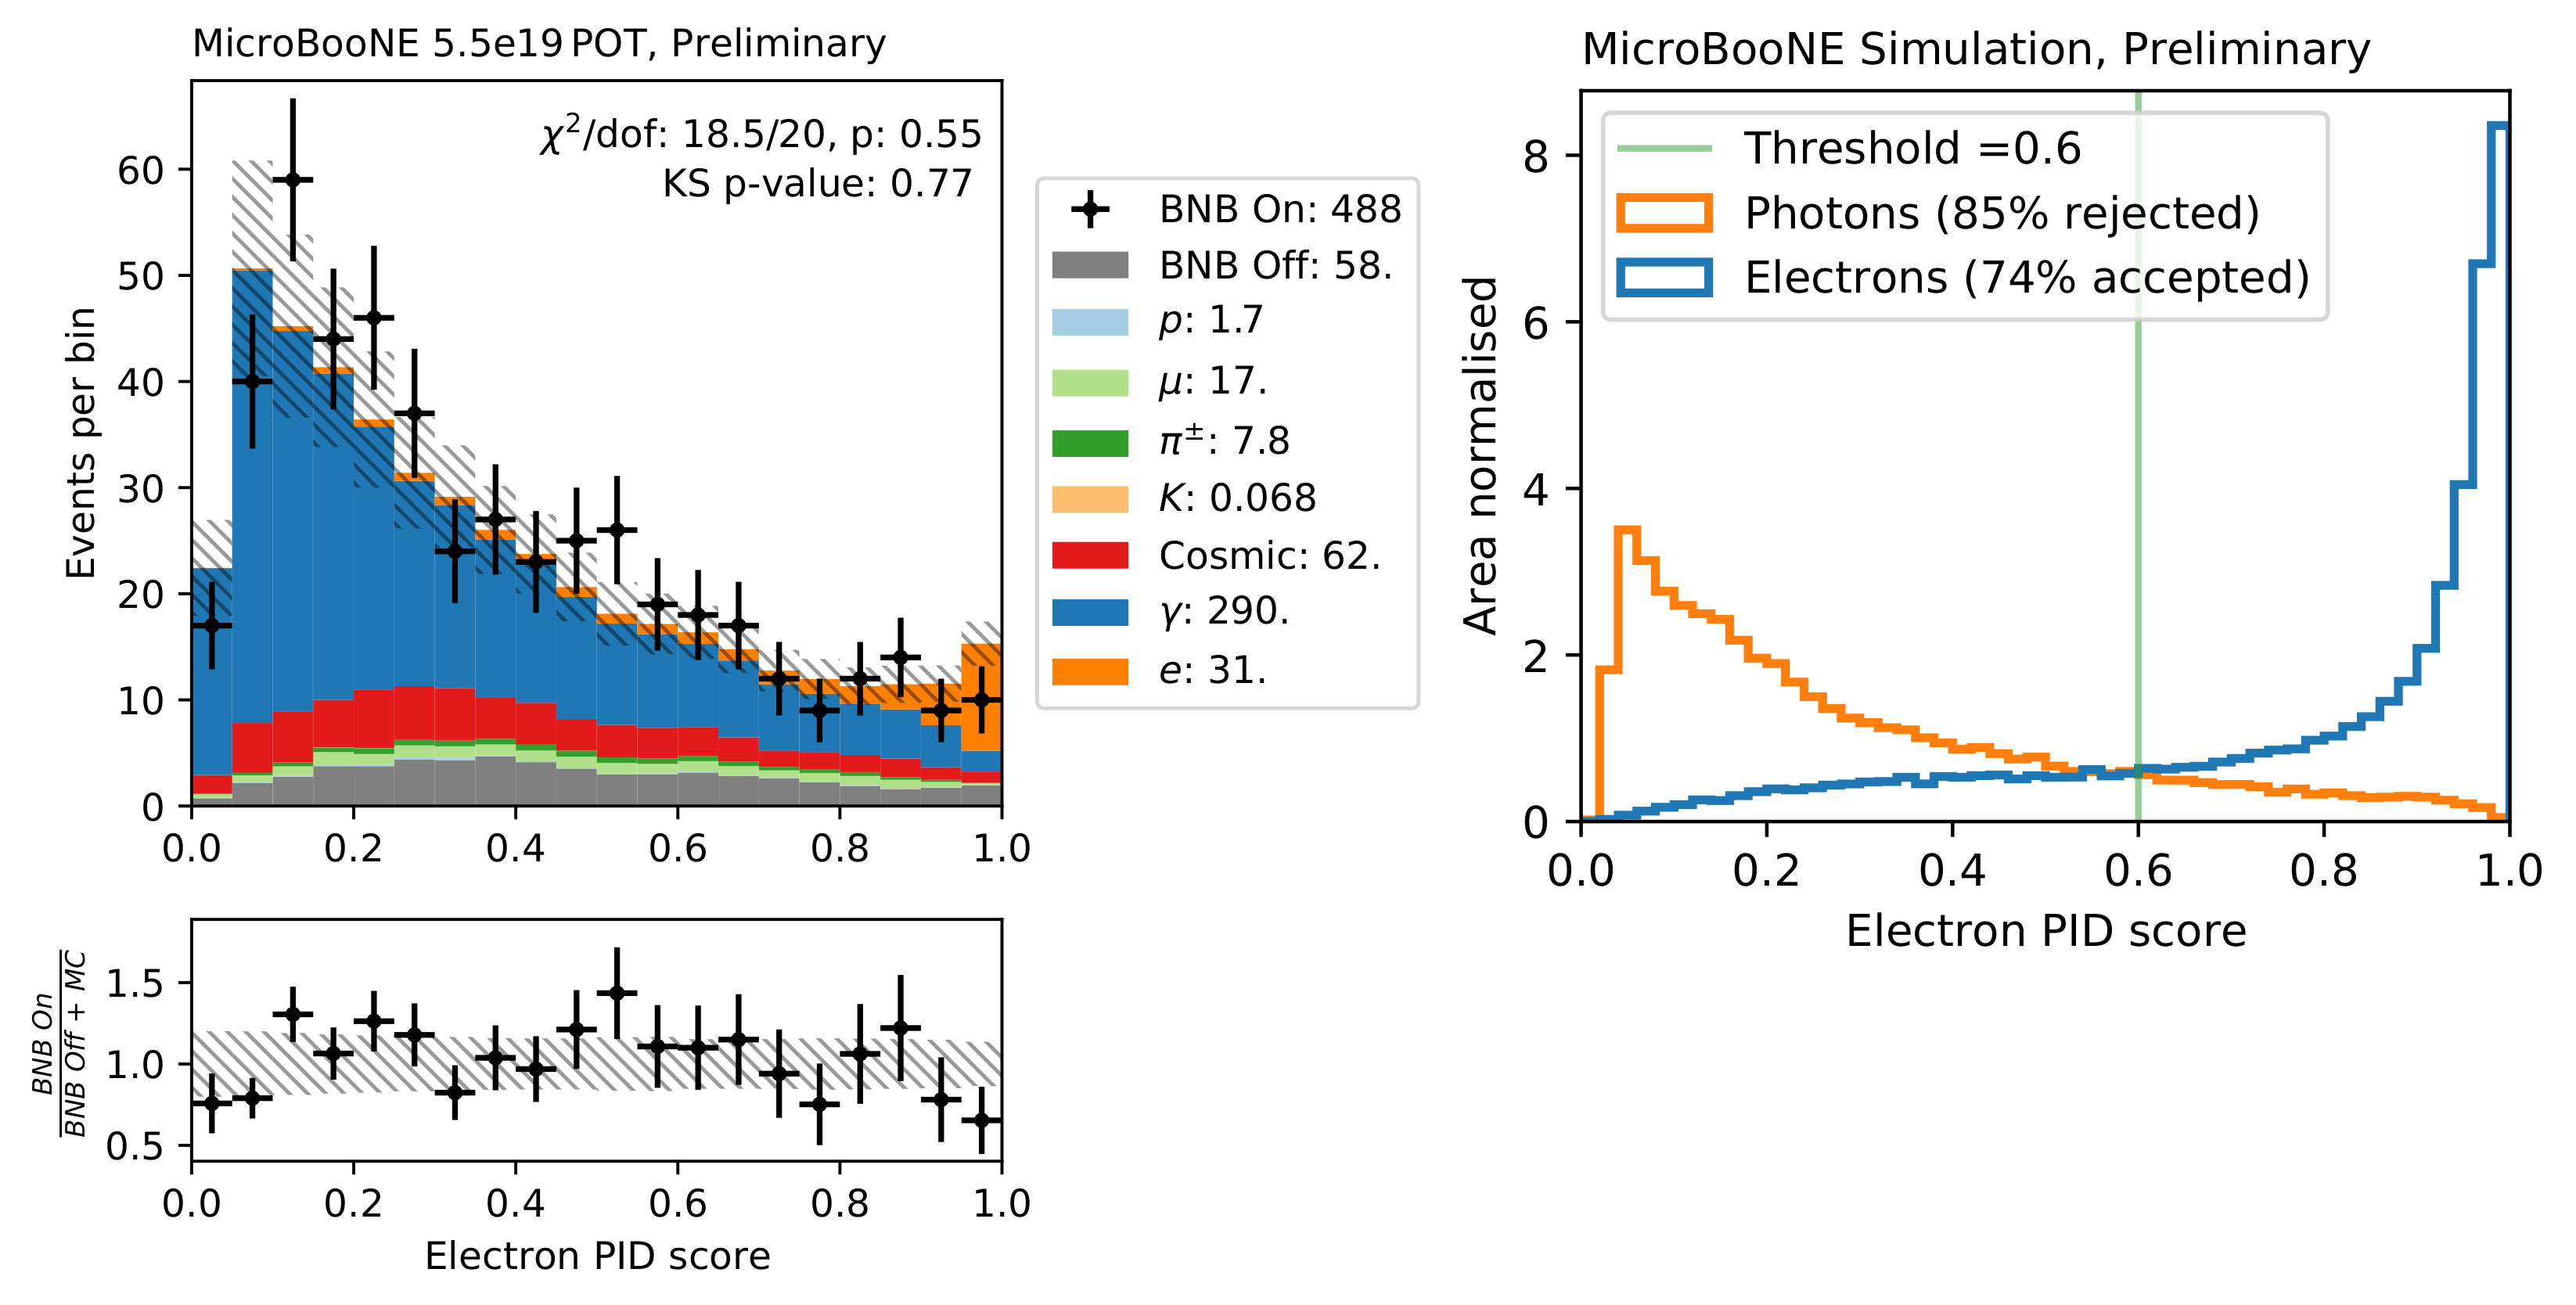
\includegraphics[height=0.27\textheight]{NueCCsel/Images/datamc/e_bdt.jpg}
\caption[$e-\gamma$ separation performance obtained by the electron classifier on simulation]{$e-\gamma$ separation performance obtained by the electron classifier on simulation. Left: the BDT response compared in data and simulation. Right: the response is shown for \nuecc electrons (blue histogram) and for background photons (orange histogram). The green line demonstrates the performance at which\pct{85} of the background photons are rejected and \pct{75} of the electrons are selected.}
\label{fig:egammasep}
\end{figure}

In \cref{fig:egammasep}, simulated neutrino events passing the \textit{pre-selection} are used to demonstrate the obtained electron-gamma separation. It is found that one can reject \pct{85} of photon showers, while keeping \pct{75} of electron showers, corresponding to a $5:1$ increase of signal-to-background ratio. This solely serves as a demonstration and no one-dimensional cut was placed on this value in the final selection. Instead, this variable is used in the final event selection as described in \cref{sc:nuecc:sel}.

\subsection{Other Daughters Identification}
\label{sc:nuecc:d_pid}

Besides the electron candidate, the reconstructed neutrino interaction can, and most likely does, include other track/shower particles. Their characteristics can be leveraged to improve background rejection (see \cref{fig:nue_flow}). These particles are referred to as \textit{``other daughters''}: they are part of the reconstructed neutrino particle hierarchy but exclude the electron candidate particle, which was discussed in the previous section.
\par 
We classify each \textit{other daughter} using a single BDT. This BDT is trained on three labelled categories: \emph{signal-like}, \emph{neutral} and \emph{background-like}. 
\begin{itemize}
\item The signal-like particles are those neutrino daughters that are backtracked to a proton or a split-off part of the electron. It is clear that these particles might be part of a \nuecc interaction and should not lead to event rejection.
\item The background-like particles are those neutrino daughters that are backtracked to a simulated muon or cosmic activity. Events that contain any of these should be rejected. 
\item The ``neutral" label accounts for trickier cases: this label is given to reconstructed particles backtracked to charged pions or photons. Charged pions should be allowed in a \nuecc search, but identification capacities between charged pions and muons in LArTPCs are limited due to their similar ionisation profile. Photons coming from neutral pions are allowed in a \nuecc inclusive search, but can help eliminating NC $\pi^0$ backgrounds too.
\end{itemize}
\par
\cref{fig:nuecc:train_d} illustrates the performance and validation of the \textit{other daughter} classification. Due to the large training sample and the small amount of variables included, the over-fitting is minimal. 
\par
The variables used to train the classifier are listed in \cref{tab:nuecc:d_bdt} an their data/MC distributions, along with the BDT response, are given in \cref{fig:nuecc:other_cand_all}.
\par
An event with multiple reconstructed particles besides the electron score will have a corresponding set of additional ``other daughter'' BDT responses. These can be aggregated for each event by taking the lowest, the average and the maximum BDT response, as given in \cref{fig:nuecc:bdt_event_input1}.

\subsection{Event Selection}
\label{sc:nuecc:sel}

The final \nuecc event classification is performed using a BDT building on the particle identification performed in the two previous sections. The variable with the strongest signal-background separation power is the electron identification response. The full list of variables is, in sequence of importance:
\begin{enumerate}
    \item Electron shower candidate BDT response (\cref{fig:nuecc:e_cand3}, right).
    \item Average score of the \textit{other daughter} identification (\cref{fig:nuecc:bdt_event_input1}, middle).
    \item Number of reconstructed shower-like particles in the event (\cref{fig:nuecc:bdt_event_input2}, left).
    \item Lowest score of the \textit{other daughter} identification (\cref{fig:nuecc:bdt_event_input1}, left).
    \item Highest score of the \textit{other daughter} identification (\cref{fig:nuecc:bdt_event_input1}, right).
    \item The number of reconstructed particles with a vertex distance of \SI{>3}{\cm} (\cref{fig:nuecc:bdt_event_input2}, middle).
    \item The containment fraction of the event (\cref{fig:nuecc:bdt_event_input2}, right).
\end{enumerate}
Completely analogous as to the particle identification BDT, \cref{fig:nuecc:train_event} illustrates the performance and validation of the event classification.
\par
The response of the event classification is given in the left panel \cref{fig:final_sel}. After the selection, the efficiency is \pct{18.1+-0.1}. The distribution of the reconstructed electron energy is given in the middle panel of \cref{fig:final_sel}. The right panel of \cref{fig:final_sel} shows the track vertex multiplicity. The latter is compared before and after selection in \cref{fig:nuecc:trk_at_vtx}. In \cref{fig:nueccinc_eff_all}, the efficiency for the three stages in the selection -- the SliceID (\cref{sc:nuecc:presel}) and the full \nuecc selection -- are given in function of the simulated neutrino energy. The efficiency is broken down for different interaction modes and final state topologies in \cref{fig:nuecc:eff}.
\par
\cref{fig:final_nue} Shows the lepton kinematics of the selected \nuecc candidates. This motivates the ability to identify, reconstruct and select electrons with relatively high-statistics and opens the door towards a cross-section measurement using BNB electron neutrino events. 
\par
A set of BNB events displays is included in \cref{fig:nue_evd}. These events are a subset of the events populating the middle and right panels of \cref{fig:final_sel} and aim to demonstrate the variety of final states and extent of the energy range that is covered by the selection. The three-plane event displays for all selected events -- with and without the reconstructed objects overlaid -- in the unblinded data are available on \href{https://drive.google.com/drive/folders/1rezW9_xjSJZkJjEk1hVKypXJPCtMGZVP?usp=sharing}{Google Drive}. The results of this selection on the far energy sideband -- reconstructed neutrino energy above $\SI{1.05}{\GeV}$ -- are discussed in \cref{sc:nuecc:sideband}.

\begin{figure}[htb]
    \centering
    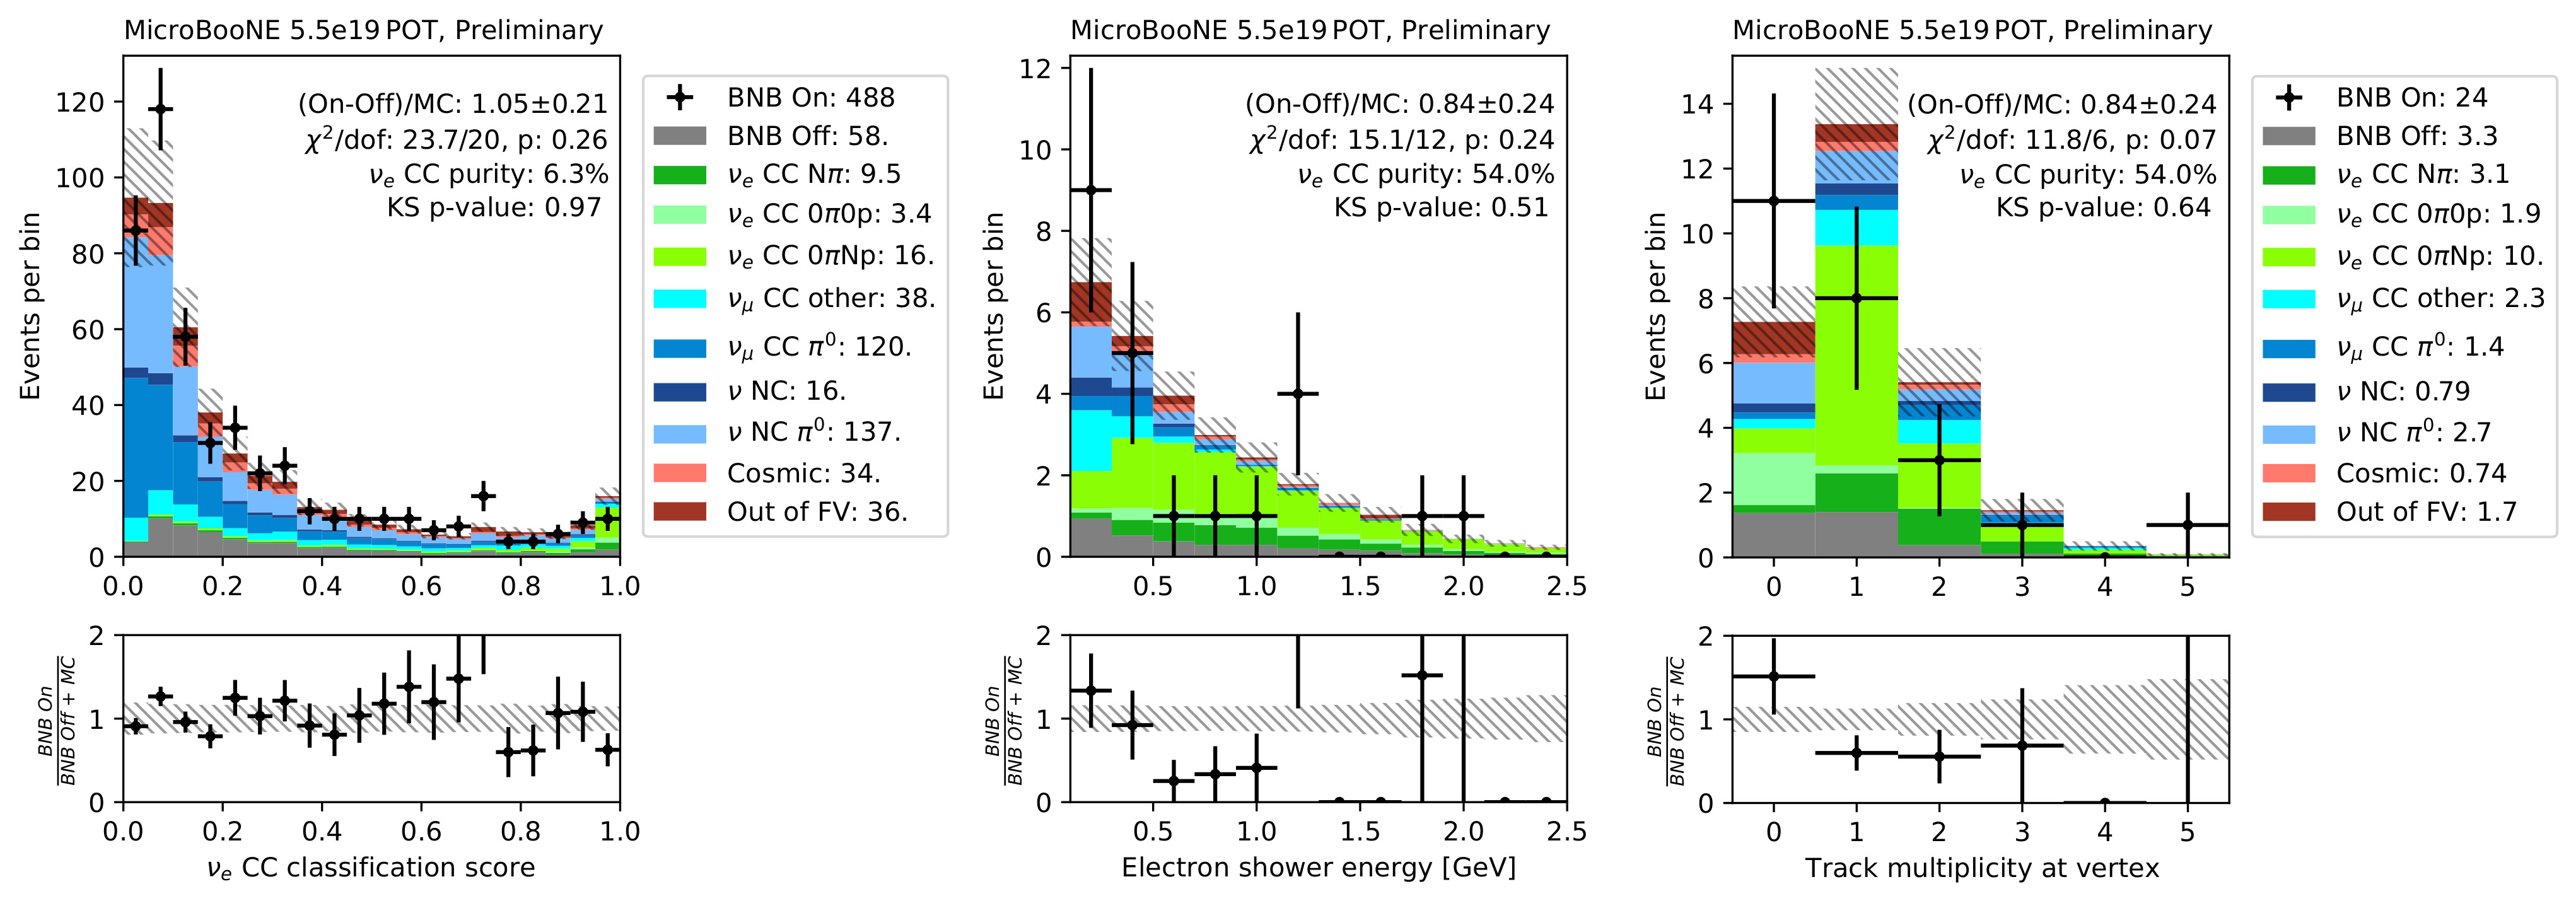
\includegraphics[width=\textwidth]{NueCCsel/Images/datamc/event_bdt_plus}
    \caption[Final \nuecc event classifier and reconstructed electron energy spectrum]{(left) BDT response of the \nuecc inclusive event classifier. (right) Reconstructed electron shower energy distribution after the selection.}
    \label{fig:final_sel}
\end{figure}

\begin{figure}[htb]
    \centering
    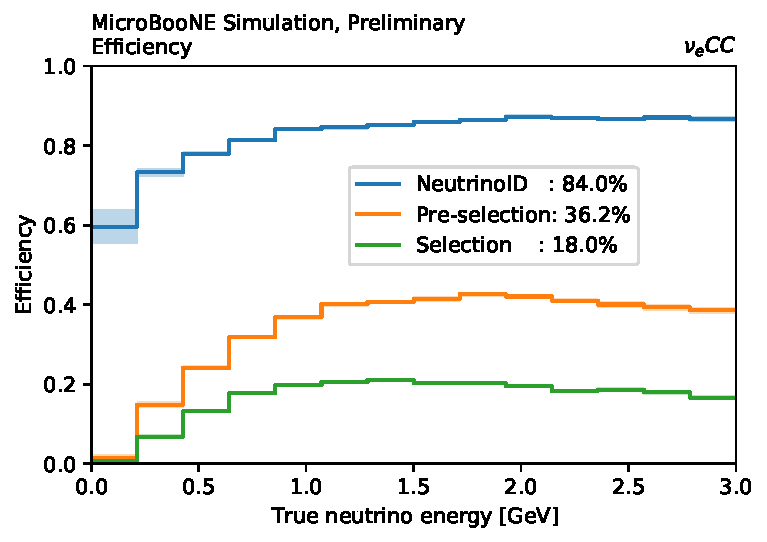
\includegraphics[width=0.4\textwidth]{NueCCsel/Images/truth/efficiency_2.pdf}
    \caption{Efficiency of the different stages in the selection in function of the true neutrino energy.}
    \label{fig:nueccinc_eff_all}
\end{figure}

\begin{figure}[htb] 
\begin{center}
    \begin{subfigure}{\textwidth}
    \centering
    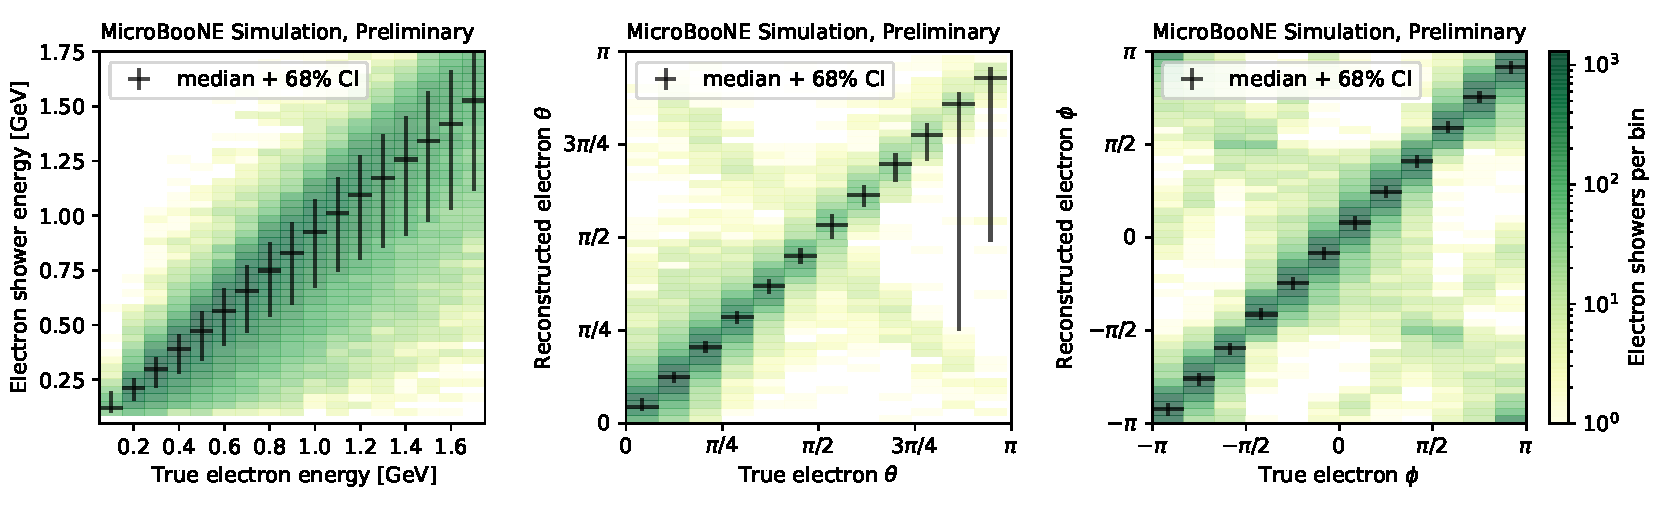
\includegraphics[width=\textwidth]{NueCCsel/Images/truth/electron_resolution.pdf}
    \caption{\label{fig:final_nue:reso}  Reconstructed resolution for the electron variables in the \nuecc selection. The colour scale for the \textit{2D} histograms is logarithmic. In black, the median and 68\% confidence interval are given, binned in the true electron kinematics.\\}
    \end{subfigure}
    \begin{subfigure}{\textwidth}
    \centering
    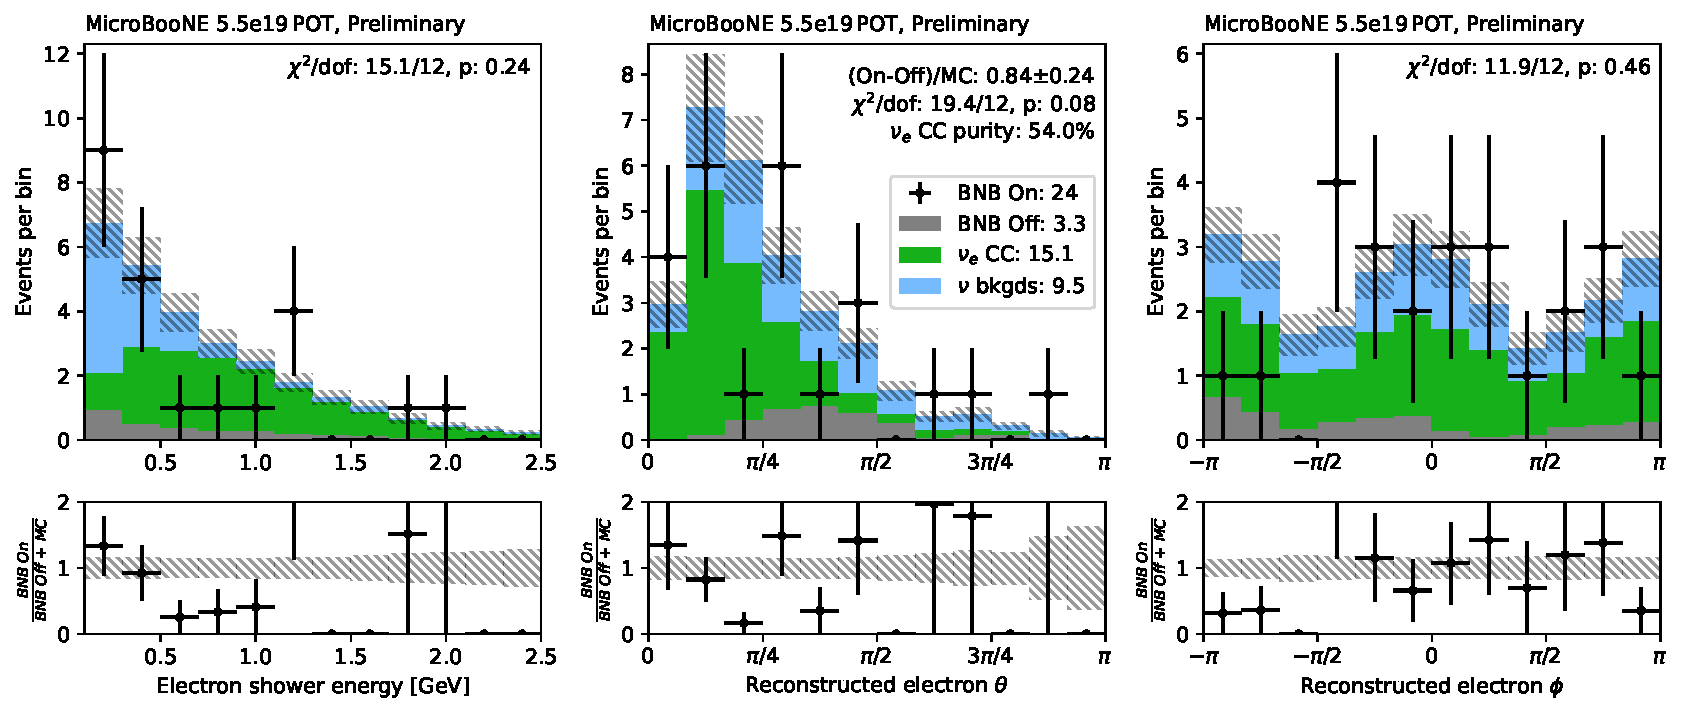
\includegraphics[width=0.94\textwidth]{NueCCsel/Images/datamc/event_e_kinematics.pdf}
    \caption{\label{fig:final_nue:datamcafter} Electron shower energy (left) and directional angles $\theta$ (middle) and $\phi$ (right) of the \nuecc electron candidate. In blue, the neutrino related backgrounds are grouped into one category. The error bars on the data are Poissonian. The errors on the prediction are the flux and cross-section \systs, combined with the uncertainty arising from the limited size of the beam off and simulated samples.}
    \end{subfigure}
\caption[Lepton kinematics for the \nuecc channel. Both resolution and data/MC comparisons are shown]{\label{fig:final_nue} \nuecc electron kinematics. Both the resolution (a) and data/MC comparisons (b) are shown. High statistics comparisons of such distributions with the full data-set distribution will provide a valuable measurement of the \nue kinematics over a broad energy range.}
\end{center}
\end{figure}

\subsection{Impact of Systematic Uncertainties}
\label{sc:nuecc:syst}

As stated in the introduction of this chapter and with be the topic of \cref{sec:systematics}, different sources of statistical uncertainty are included:
\begin{enumerate}
    \item Flux uncertainties: incorporated with the covariance matrix using 1000 universes (\cref{sec:systematics:flux}).
    \item Cross-section modelling: incorporated using 500 universes and 7 up/down unisim variations. The latter are taken into account on the diagonal of the covariance matrix. For one of the unisim GENIE variations, the \textit{CCMEC}, the required sample was unavailable at the time of writing and will be incorporated in the next iteration (\cref{sec:systematics:xsec}). 
    \item Re-interactions in liquid argon (Geant): incorporated using 1000 universes using the covariance matrix formalism.
    \item Finite simulation(overlay) and external (\textit{BNB Off}) statistics: incorporated on the diagonal of the covariance matrix% (\cref{sec:systematics:stat}).
    \item Detector variations: The effect of 11 detector effects are studied. Their effect on the selection efficiency is shown in \cref{fig:nuecc:detvar_eff} and is at the sub-percent level. Nevertheless, as shown through three examples in \cref{fig:nuecc:detvar_ex}, the detector variation can lead to important shape differences .%(\cref{app:detsys}). 
\end{enumerate}
The full covariance matrix is constructed by summing the contributions from the universes. The unisim variations are added in quadrature to the covariance matrix diagonal. The effect of the different sources of \systs on the normalisation is broken down by source in \cref{tab:nuecc:syst}. 

\begin{table}[htb]
    \centering
    \begin{tabular}{llc}
\hline
Source                 & Type           & Impact on normalisation [$\%$] \\ \hline
Flux                   & 1000 universes & 5.69                           \\
Cross-section          & 500 universes  & 14.2                \\
Re-interaction         & 1000 universes & 0.70                           \\
ThetaDelta2Npi         & up/down        & 2.58                           \\
RPA                    & up/down        & 0.74                           \\
DecayAngMEC            & up/down        & 0.06                           \\
AxFFCCQE               & up/down        & 0.05                           \\
VecFFCCQE              & up/down        & 0.19                           \\
CCMEC                  & up/down        & ?                              \\
Detector Variations    & unisim         & 3.33                           \\
Monte-Carlo statistics &                & 1.51                           \\ \hline
\end{tabular}
    \caption{Effect of different \systs on the normalisation (single-bin) after the \nuecc selection. The CCMEC knob was unavailable at the time of writing and will be added later. It is clear that the overall \syst is dominated by the cross-section modelling.}
    \label{tab:nuecc:syst}
\end{table}

\begin{figure}
    \centering
    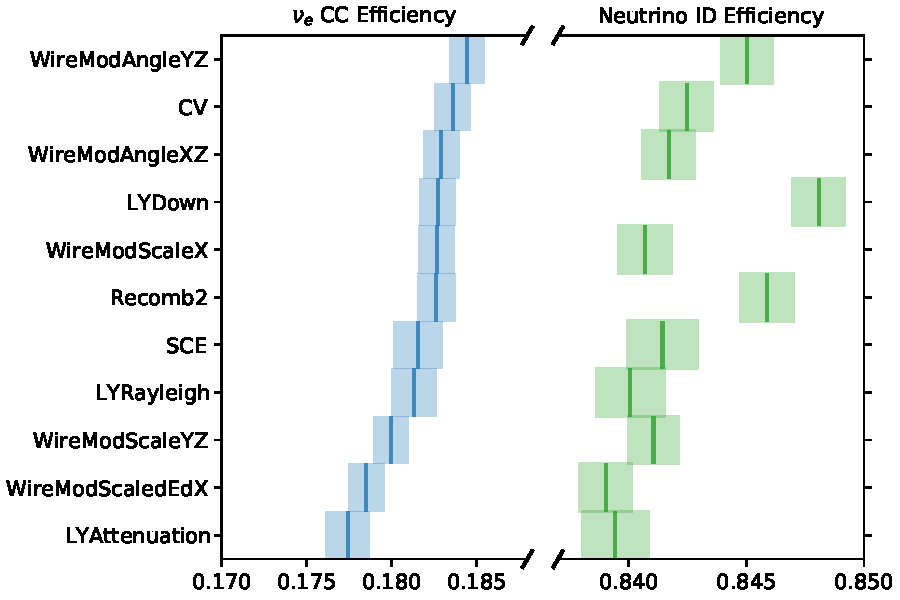
\includegraphics[width=0.5\textwidth]{NueCCsel/Images/syst/efficiency.pdf}
    \caption{Effect of the detector variation on the selection efficiency at the NeutrinoID and final selection stage. The shaded areas correspond to statistical variations due to the finite size of the unisims. Note that the light-yield attenuation sample is currently an over-estimating and is therefore not included in the covariance matrix construction.}
    \label{fig:nuecc:detvar_eff}
\end{figure}

\begin{figure}
    \centering
    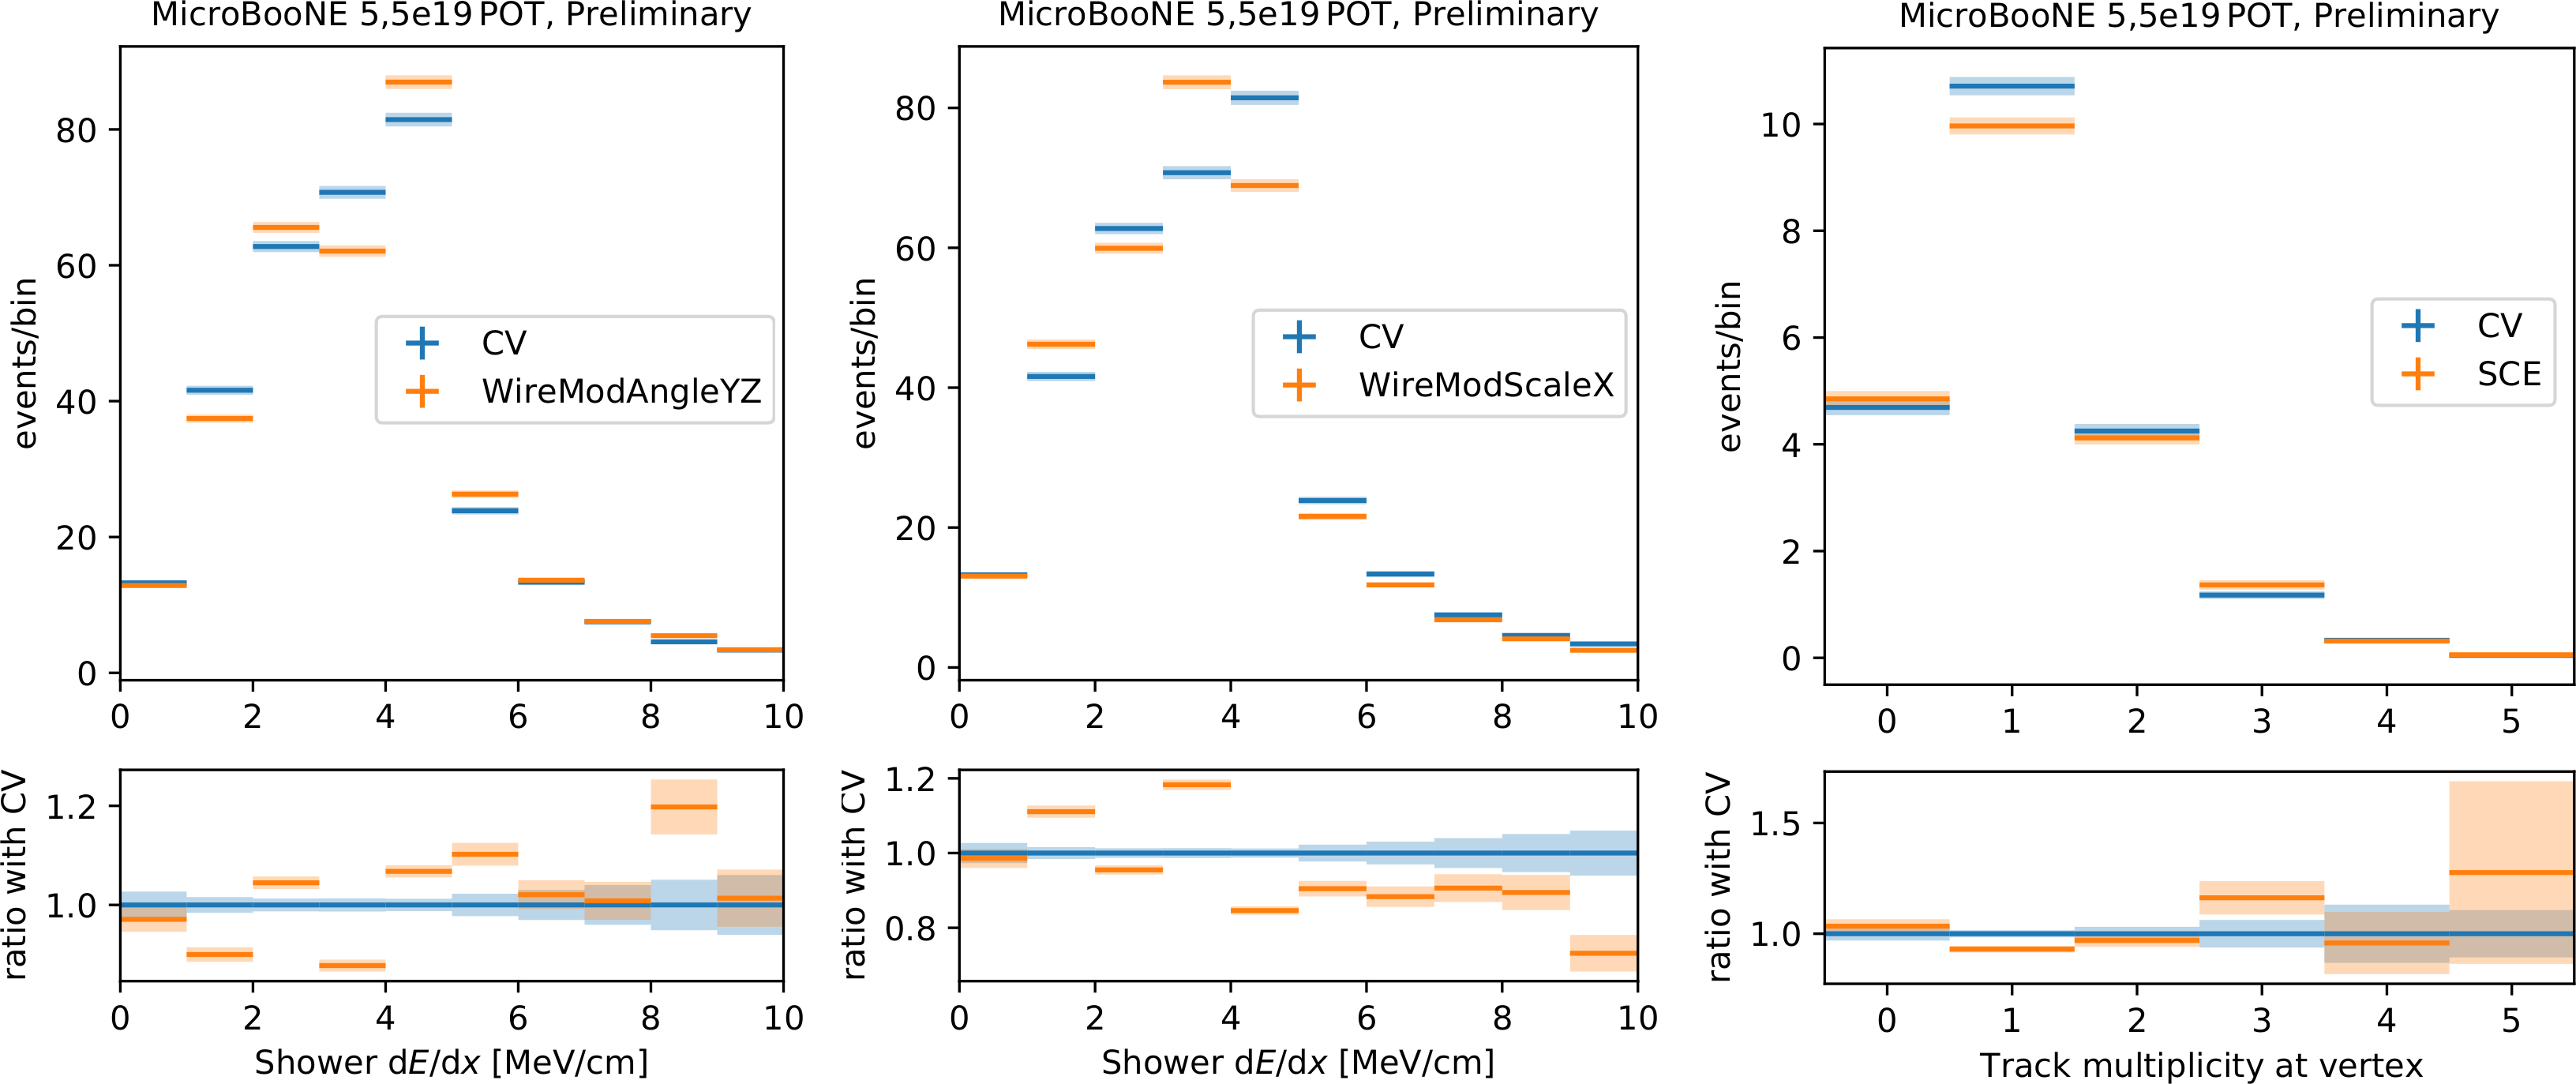
\includegraphics[width=\textwidth]{NueCCsel/Images/syst/syst_variations.png}
    \caption{Three examples of bin-by-bin variations introduced by detector variations. The effect of two wire modification samples on the shower \dedx at preselection is shown in the left and middle panels. The variations are in opposite direction and have a sizable impact on the separation of the double-peaked $e$/$\gamma$-structure. The right panel illustrates the effect of the space charge variation on the vertex multiplicity after selection. The expected number of events with a single track is significantly lowered, similar to data shown in \cref{fig:final_sel,fig:nuecc:sideband:trk_vtx}. }
    \label{fig:nuecc:detvar_ex}
\end{figure}


\begin{figure}[htb]
    \begin{subfigure}{\textwidth}
    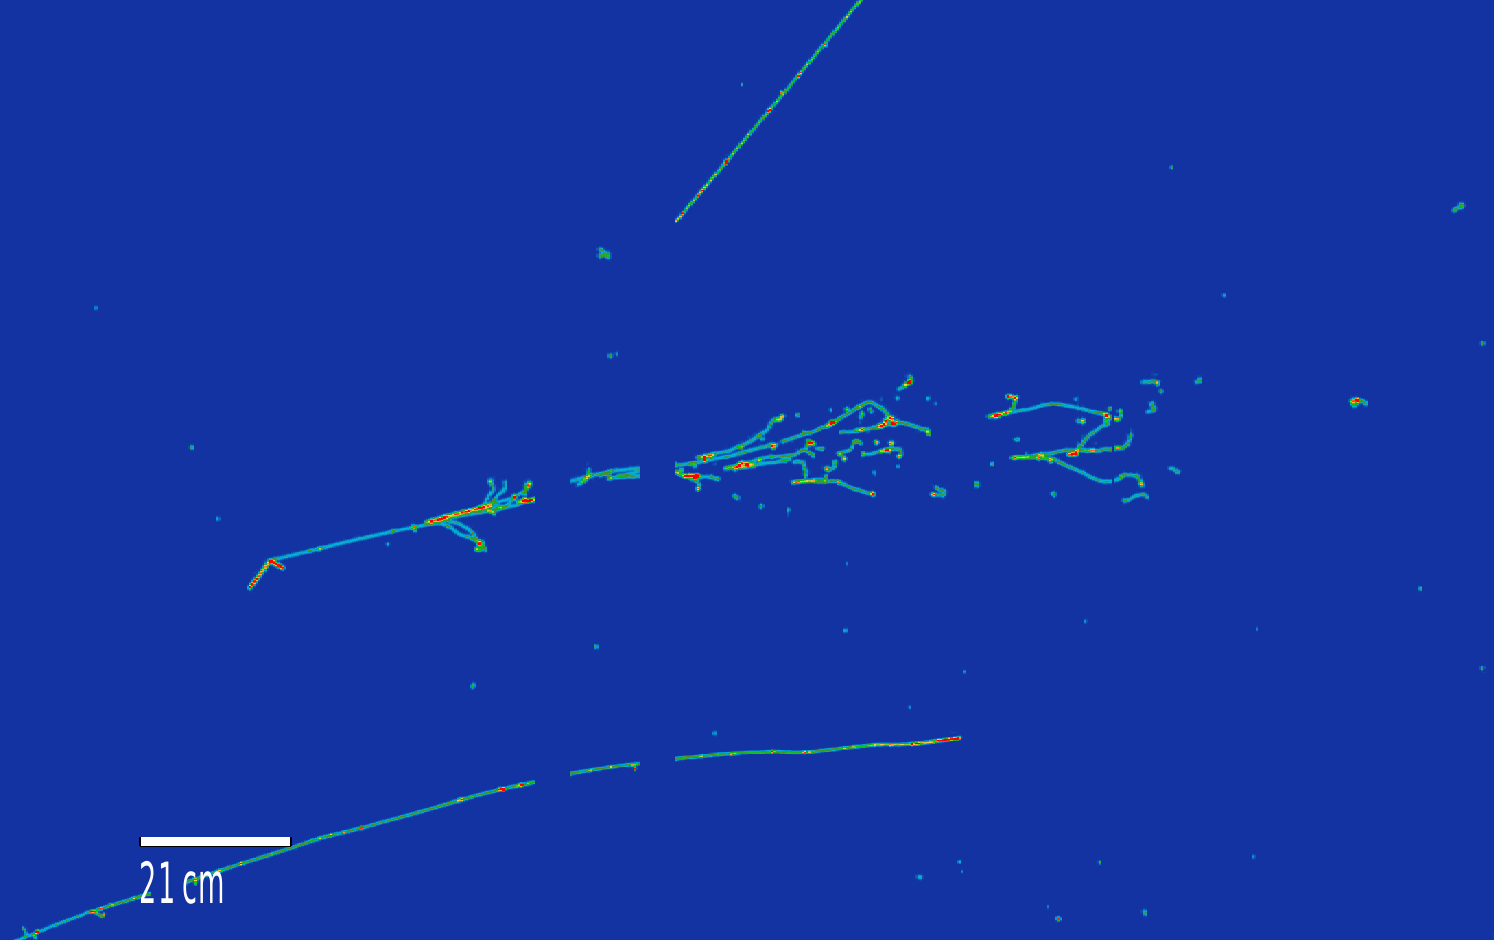
\includegraphics[width=0.46\textwidth]{NueCCsel/Images/evd/nue_5161_8_447}\hfill 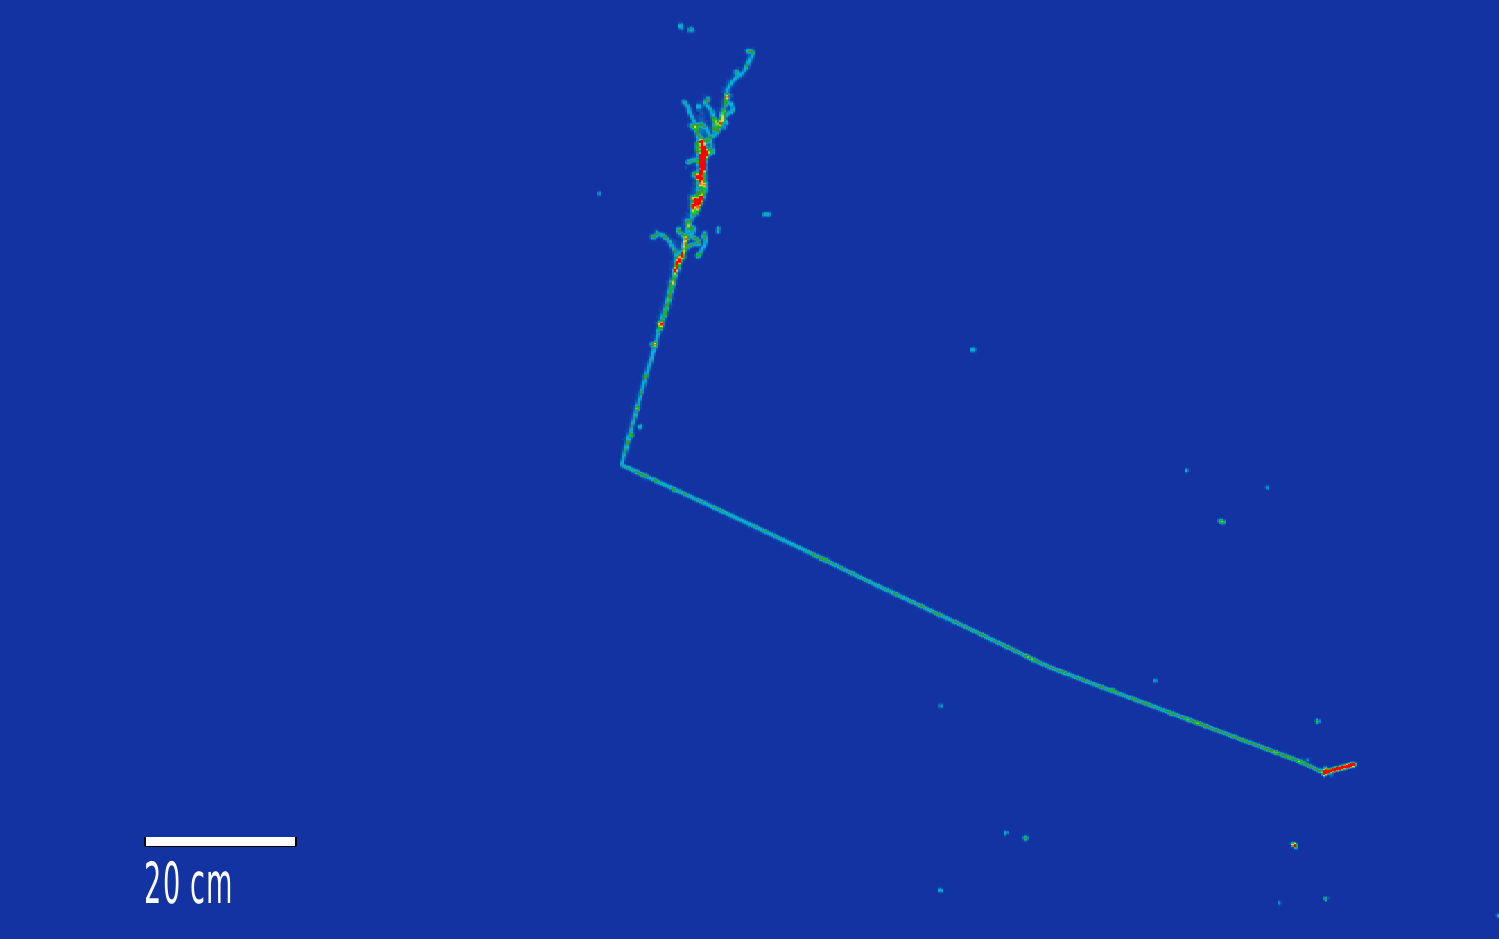
\includegraphics[width=0.46\textwidth]{NueCCsel/Images/evd/nue_5360_0_45}
    \vspace{1mm}
    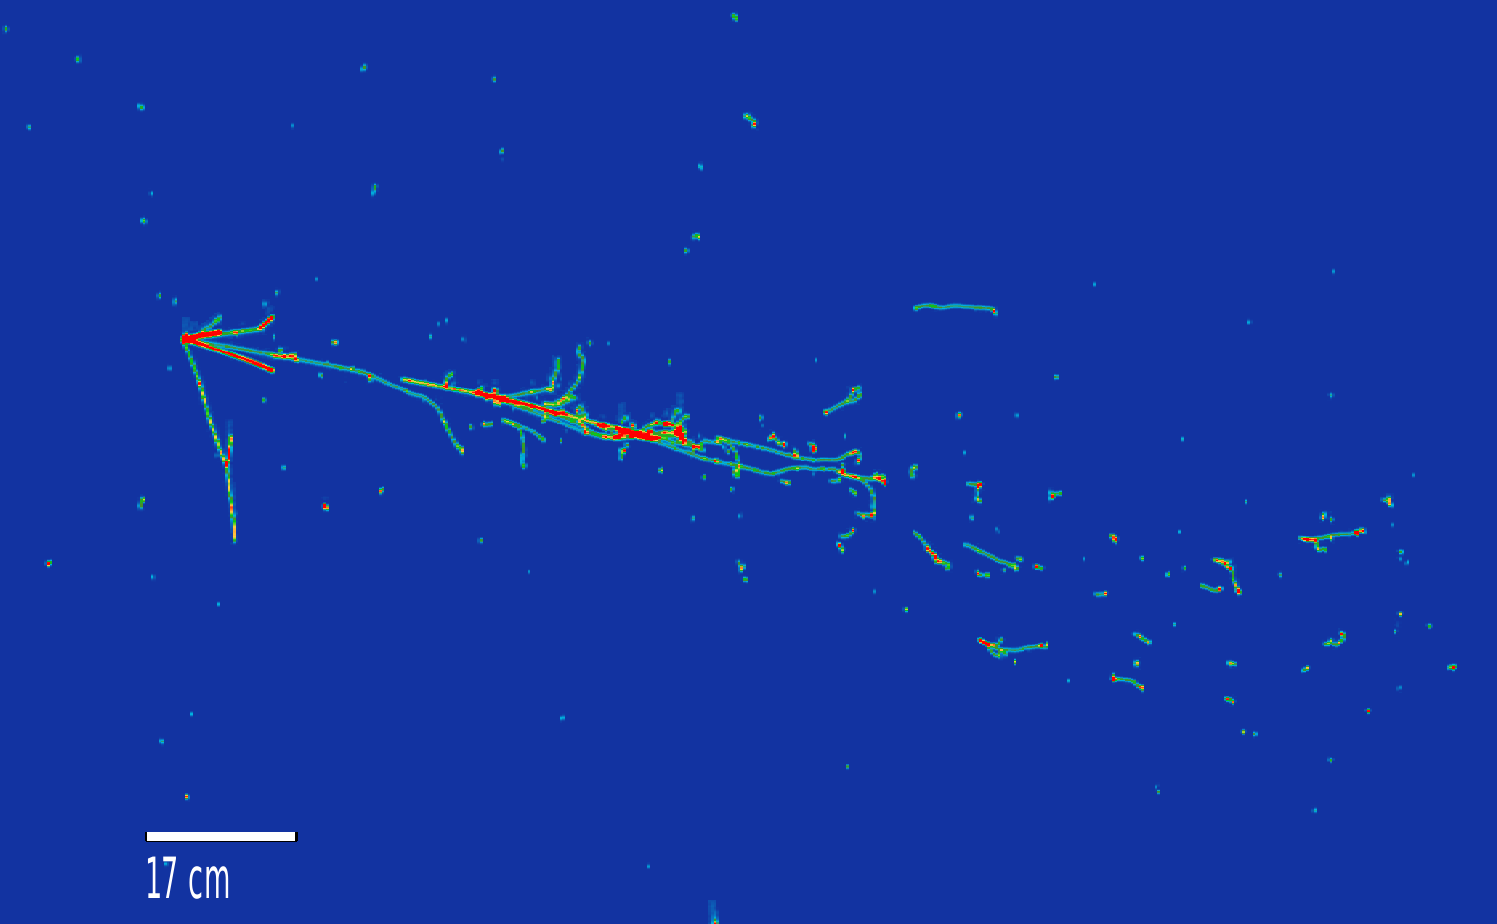
\includegraphics[width=0.46\textwidth]{NueCCsel/Images/evd/nue_5444_87_1}\hfill 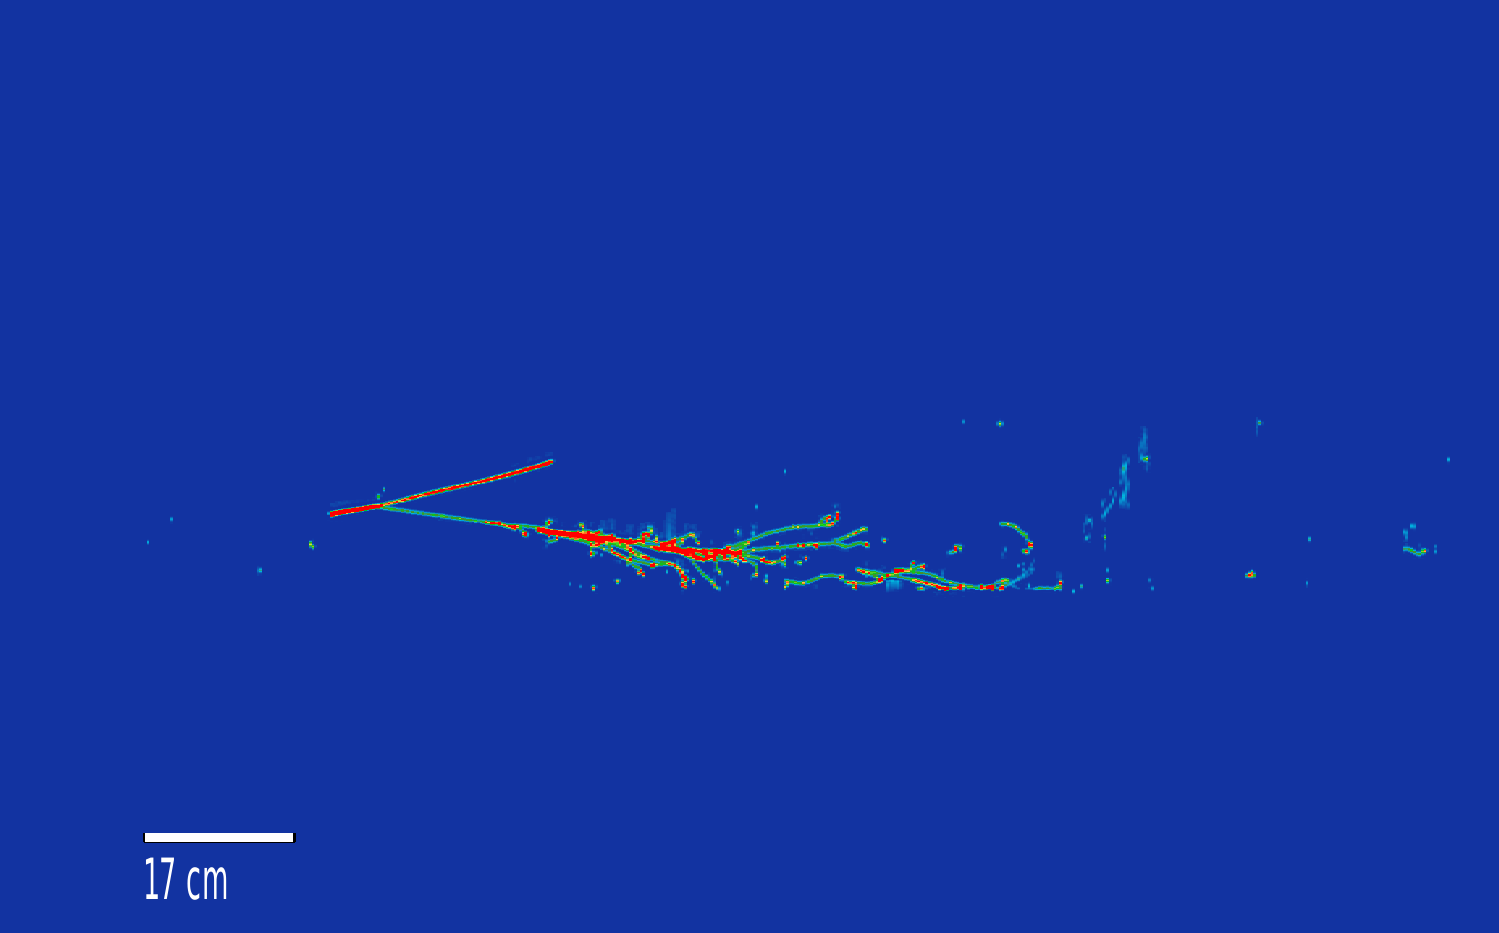
\includegraphics[width=0.46\textwidth]{NueCCsel/Images/evd/nue_5583_13_692}
    \vspace{1mm}
    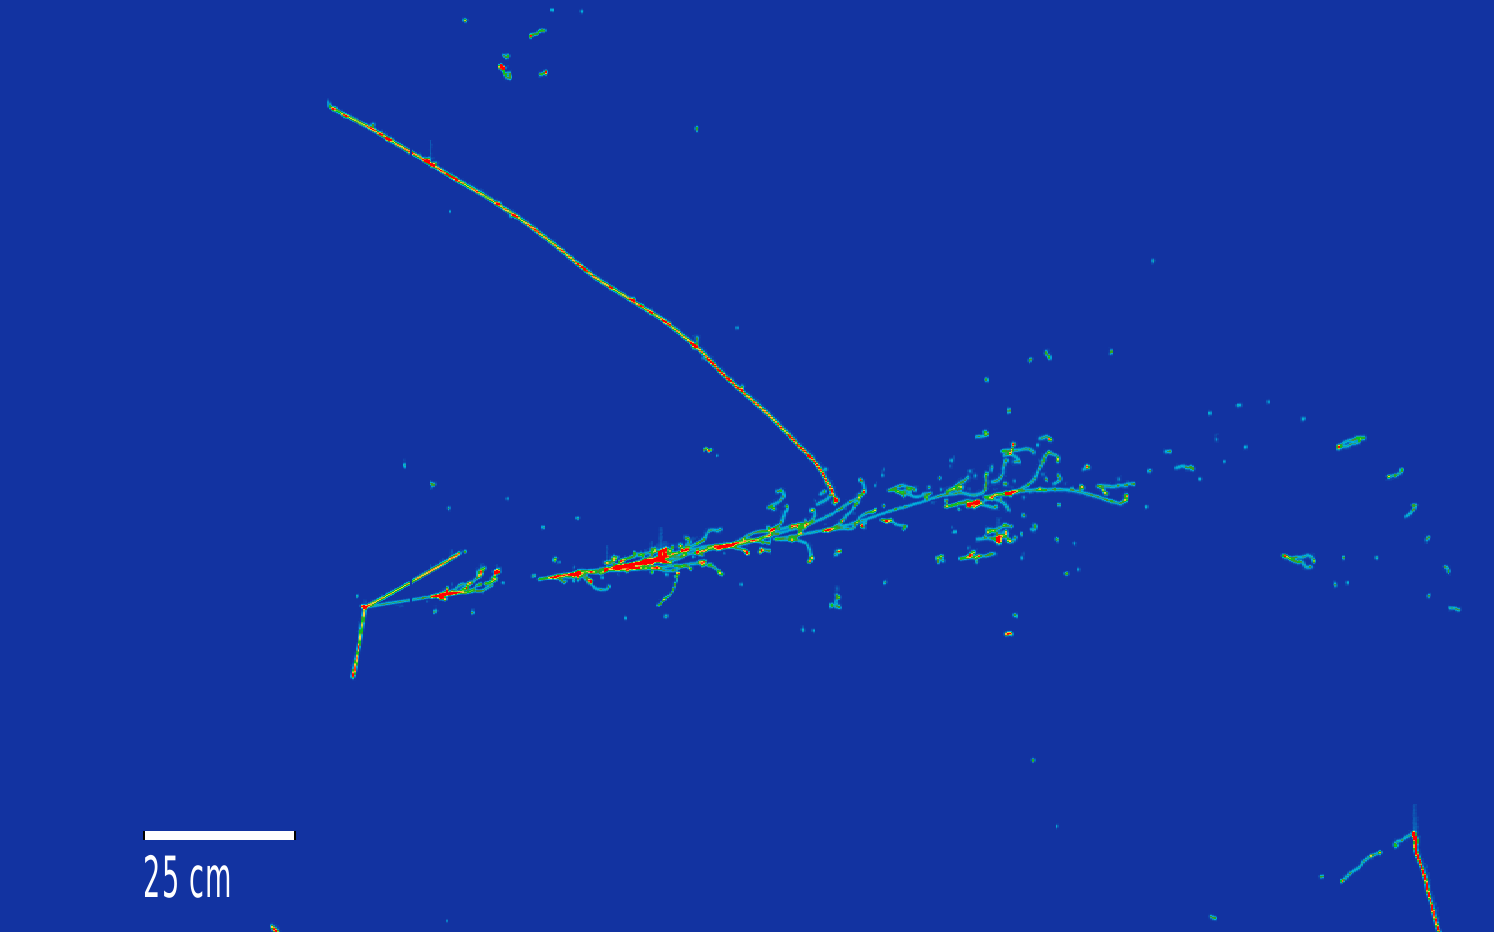
\includegraphics[width=0.46\textwidth]{NueCCsel/Images/evd/nue_5607_15_796} \hfill 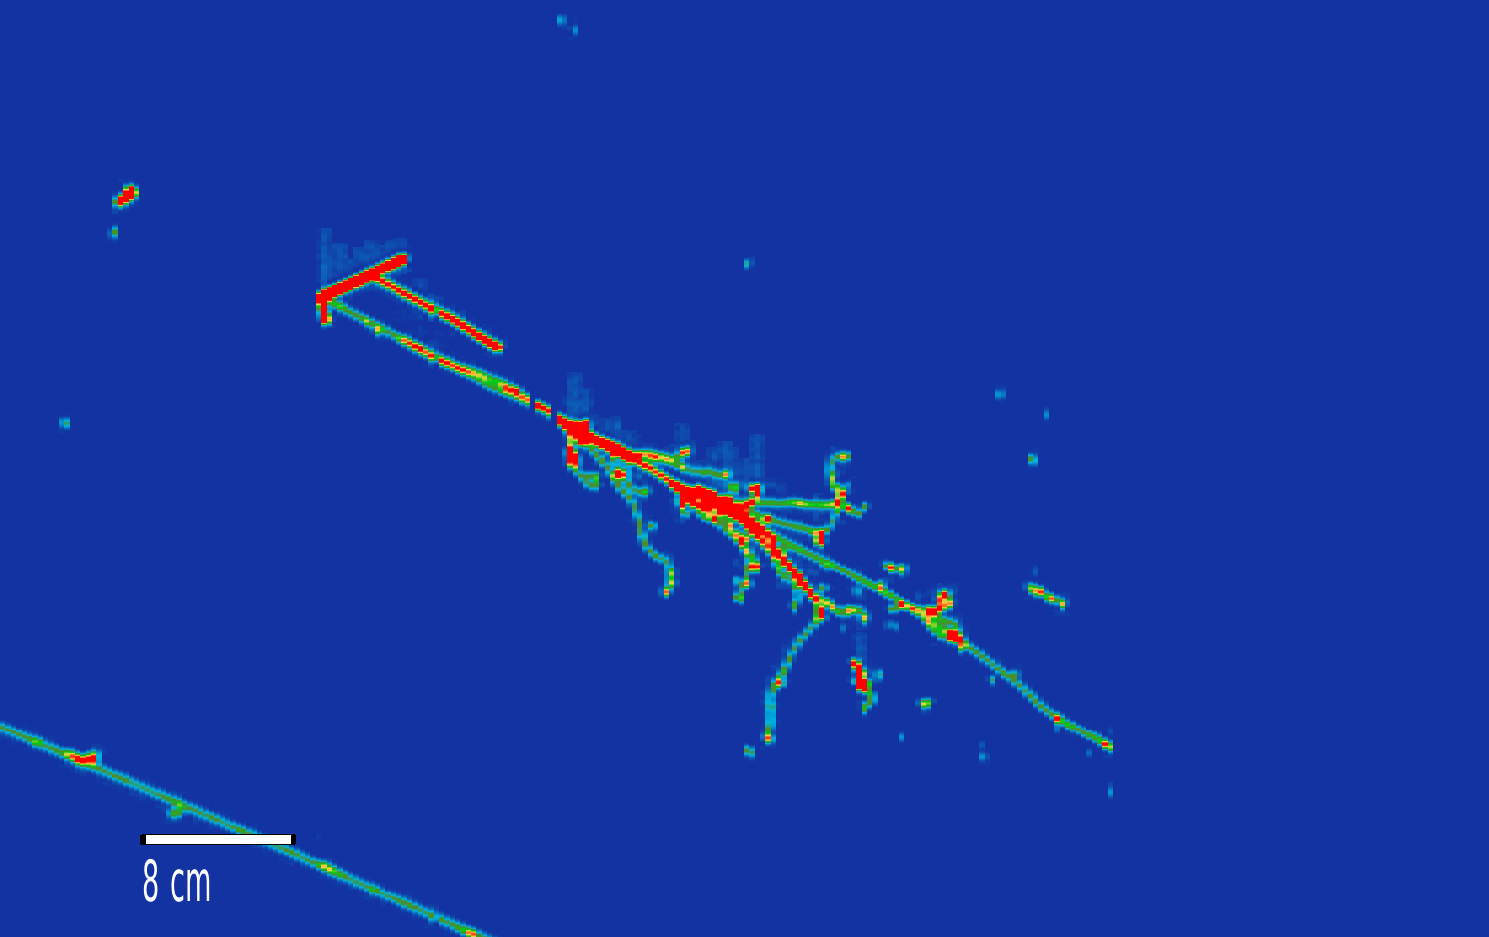
\includegraphics[width=0.46\textwidth]{NueCCsel/Images/evd/nue_5729_121_6086}
    \caption{\label{fig:nue_r1} Selected \nuecc candidates as observed in the collection plane, Run1 (\SI{4e19}{POT}) data-set. Reconstructed shower energies, from left to right, top to bottom: \SIlist{965;204;1086;989;1444;754}{\MeV}\\}
    \end{subfigure}
    
    \begin{subfigure}{\textwidth}
    \centering
    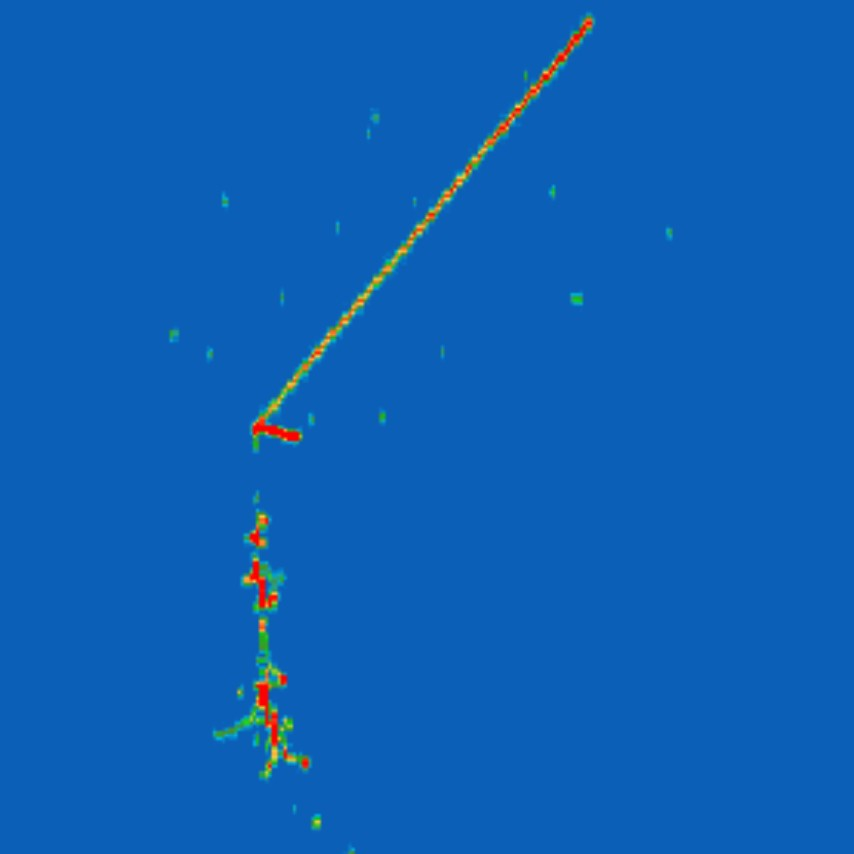
\includegraphics[width=0.3\textwidth]{NueCCsel/Images/evd/r3u}
    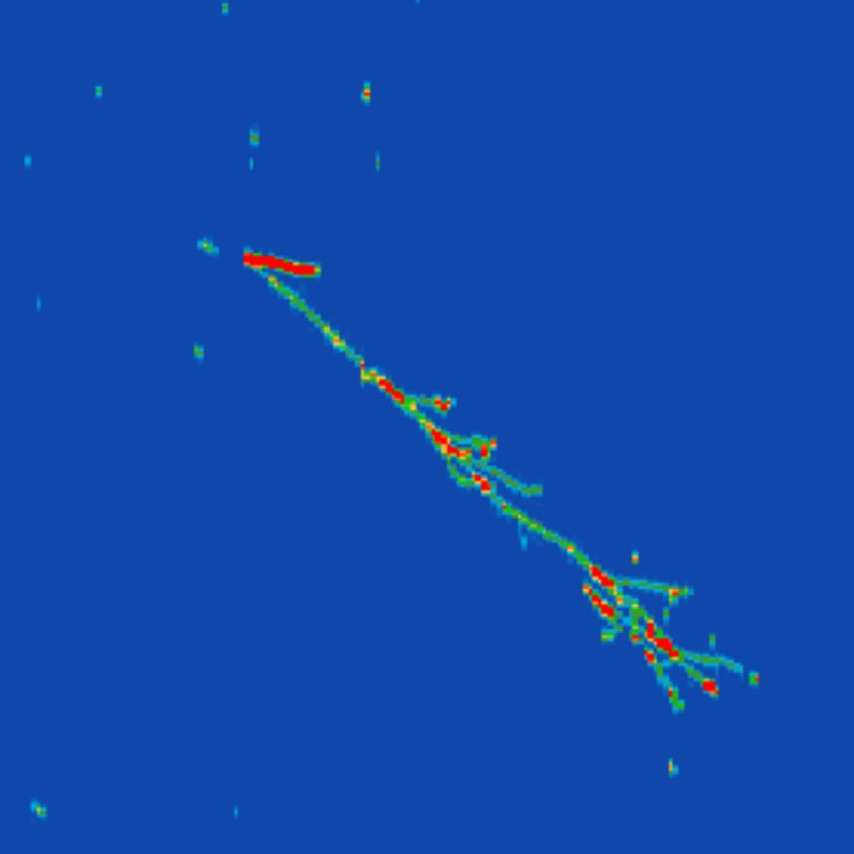
\includegraphics[width=0.3\textwidth]{NueCCsel/Images/evd/r3v}
    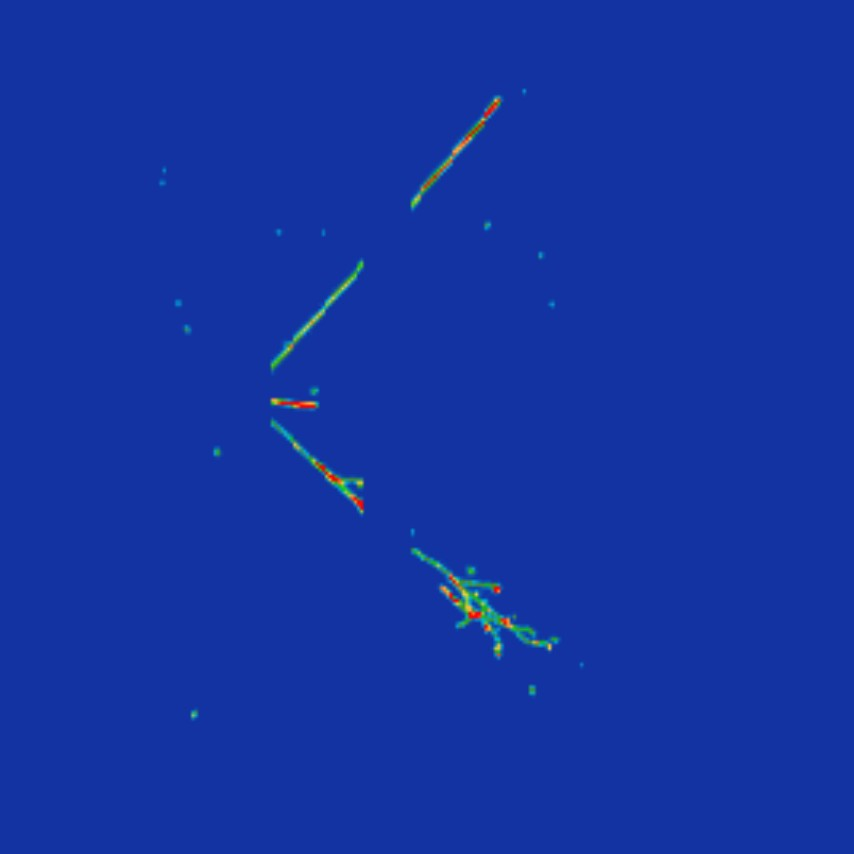
\includegraphics[width=0.3\textwidth]{NueCCsel/Images/evd/r3y}
    \caption{\label{fig:nue_r3} MicroBooNE electron neutrino candidate from the \SI{9e18}{POT} Run3 data-taking period. The reconstructed shower energy is \SI{297}{\MeV}. The three planes, $U$, $V$ and $Y$ are given from left to right.}
    \end{subfigure}
    
	\caption{\label{fig:nue_evd} Displays of selected \nuecc candidate events by the selection described in this chapter.}
\end{figure}